\chapter{Literature Review}
\label{Chapter:Literature-Review}

As it was mentioned in Chapter \ref{Chapter:Introduction} this document proposes a system implemented on a mobile device that encourages the reduction of sedentary time via self-management techniques. In order to gain knowledge on how to devise such as system, literature review needs to be carried away on several topics. First of all, the current shift towards self-management in the health sector will be discussed. The next section will focus on evaluating how much time people spend in Sedentary Behaviour (SB) and what are the consequences. Section 3 looks at digital behaviour change techniques. Commercial and non-commercial \gls{har} mobile applications and \gls{har} itself are discussed in Section 4. Section 5 summarises the system proposed.

\section{Self-Management in the Health Sector}
 \label{section:sm-in-hs}
    Mobile devices with embedded self-management logic are currently being utilised and becoming a well-accepted solution for millions of people in the health sector. For example, the NHS’s England Executive – Simon Stevens, launched a programme “Test Beds” \citep{nhsengland2016,nhsengland2016a} which is a set of collaborative projects between NHS and some technology companies such as Verily, IBM and Philips. The idea behind the project is to test the effectiveness of different technological innovations, including wearable devices and mobile applications. These technologies will enable patients to self-manage illnesses such as diabetes, heart diseases and dementia.
    
    \subsection{Advantages of self-management}
    Shifting towards self-care via mobile devices has many advantages over the traditional methods (e.g., over the phone or face-to-face). For example, self-care devices enable patients to monitor their illnesses at home. \citet[10]{roberts2006} finds that patients using wearables improve their condition and shorten their recovery time if they can be in a familiar environment. Real-time feedback is another advantage of using self-management devices. For example, \citet{alivecor2016}, can prevent critical and even fatal incidents by identifying illness clues ahead of time. Thus, the number of patients becoming seriously ill or needing hospital treatment will potentially be reduced. Consequently, that could save money on hospital treatments \citep{campbell2016}. In addition, \citet[6]{shuger2011} found that real-time feedback on \gls{sb} could be beneficial for weight loss. \citet[97]{whitehead2016} concludes that self-management approaches delivered via mobile applications have the potential to improve outcomes of many chronic diseases.
    
    \subsection{Need for self-management devices}
    It has been found that there is a gap in the current market regarding self-care devices that focus on monitoring \gls{sb} and not only \gls{pa}. For example, \citet{sanders2016} found out that there is a lack of self-management mobile applications or devices on the market that can monitor \gls{pa}. After research, he was able to find 73 devices that provide self-monitoring of PA, and only 9 can monitor sedentary time (see Figure \ref{fig:devices-to-provide-SB-feedback}). That means that there is a lack of products in the market that offer self-management of SB in addition to PA. Sanders also concluded that the current devices capable of measuring sedentary time and providing feedback have not been used in behaviour change interventions. In conclusion, there is a need for further research and development of self-care enabled wearables to help people engage in behaviour change interventions and prevent possible chronic diseases. 
    
    \begin{figure}[h]
        \centering
        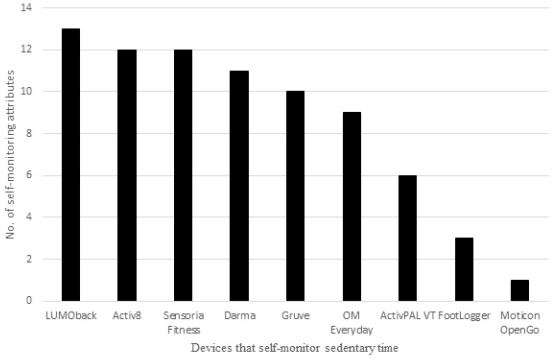
\includegraphics[width=10cm]{figureOne}
        \caption{Current technologies that self-monitor and provide feedback on SB \citep{sanders2016}}
        \label{fig:devices-to-provide-SB-feedback}
    \end{figure}

\section{Sedentary Behaviour}

Understanding the consequences of \gls{sb} as well as recommended daily energy expenditure levels is crucial for developing a mobile application that aims to implement behaviour changing theory. It is said that there is a difference between \gls{sb} and \gls{pa} and these terms should be treated differently \citep[540]{networ2012}. For example, a person can do both be sedentary for prolonged periods of time and spend large amounts of vigorous physical activity in one day. Networ define \gls{sb} as “energy expenditure less or equal to 1.5 METs while in a sitting or reclining posture” (see Table 1 for comparison of different activities). As it can be seen from Table \ref{fig:activity-intensities}, the energy spent in static activities does not result in a lot of energy expenditure and that potentially could lead to the occurrence of chronic diseases. \citet[540]{networ2012} also defines a person who is “inactive” as “not meeting specified physical activity guidelines”. That means that a person has to meet the PA recommendation levels in order to be considered as active. The next section will discuss the consequences of SB and the suggested amount of physical activity per day.

    \begin{figure}[h]
        \centering
        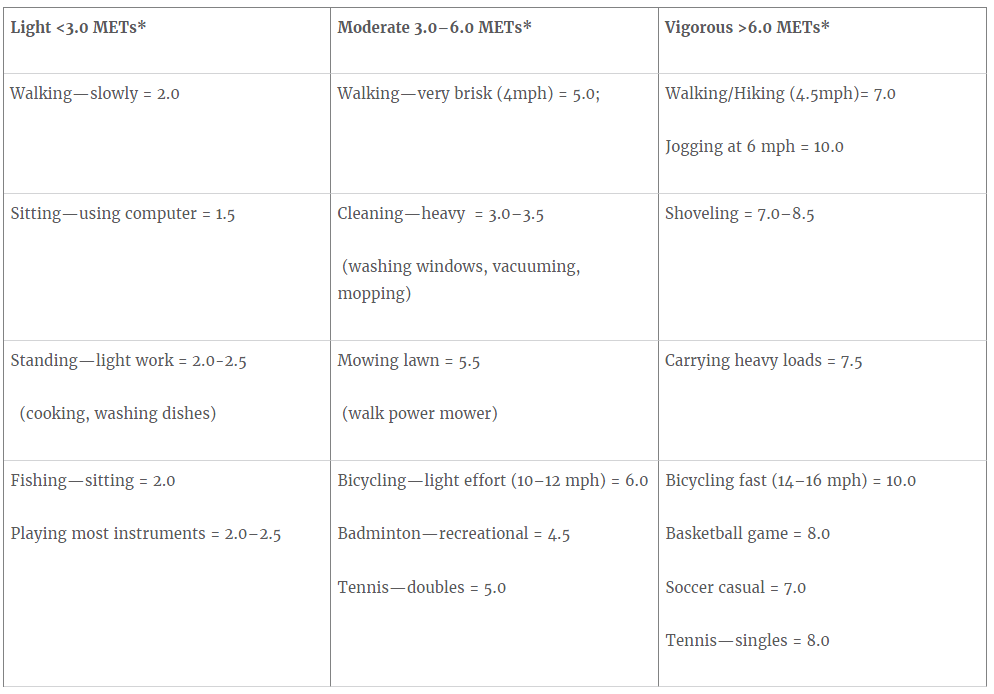
\includegraphics[width=10cm]{tableOne}
        \caption{Examples of light, moderate, and vigorous activities \citep{harvardthchanschoolofpublichealth2012}}
        \label{fig:activity-intensities}
    \end{figure}
    
    \subsection{SB consequences and PA recommendations}
    Sedentary Behaviour has been positively associated with diseases such as back pain, diabetes, cardiovascular disease, cancer and all-cause mortality (Wilmot et al., 2012: 2895–2905, Biswas et al., 2015: 123 and Department of Health, 2010: 18). In addition, Biswas et al. (2015: 127) even concluded that SB causes adverse outcomes regardless of the physical activity, although the chances of developing a SB associated chronic diseases are low when involved in higher levels of physical activity.
    
    As far as the PA recommendations are concerned, the Department of Health (2011) and Townsend et al. advocate for 30 minutes of PA for every day of the week. What is more, Parkinson (2016) and Siddique (2016) state that an ideal PA per day would be an hour. Having said that, simply doing 30 minutes or even an hour of activity is not enough. For example, a person may do 30 minutes of activity a day and spend the rest of the time laying or sleeping. To counter that, Swartz, Squires, and Strath (2011) suggest that every static hour should be interrupted by at least of a five-minute walk.
    
    \subsection{Current statistics of sedentary behaviour}
    \citet[19]{townsend2015} found in 2012 that 34\% of adult man and 46\% of adult women did not meet the recommended levels of physical activity. Also, according to \citet[81]{townsend2015}, 45\% of the adults in the UK spend up to 5h and 30 minutes in SB such as watching TV, using a computer or playing video games. What is more, \citet{swinford2014} found in a survey that there has been an increase in the time people spend in sedentary activities compared to 1995. For example, he found that people nowadays take 18 per cent fewer journeys, 24 per cent fewer go to do shopping and 28 per cent visit friends compared to 1995. In conclusion, to improve the state of the people who are spending too much time in sedentary behaviour, there is a need for further research on the effectiveness of behaviour change interventions only focusing on sedentary time and physical activity alone \citep[130]{biswas2015}.

\section{Behaviour change}
Behaviour change is a critical aspect of self-management. It could encourage and motivate people who spend too much time being sedentary to improve their lifestyle. Behaviour change includes the following main components: goal-setting, monitoring and feedback. \citet[191]{strecher1995} find that setting a specific goal, combined with performance feedback, increases task performance (how well a task is achieved) when compared to having no goal or non-quantitative goal such as “do you best”.

Providing feedback is also important in order to successfully implement behavuour change. \citet[708]{locke2002} gives the following example “If the goal is to cut down 30 trees in a day, people have no way to tell if they are on target unless they know how many trees have been cut”. A person needs to know how much effort they need to put in order to attain a previously set goal. This information is provided by the monitoring component of the behaviour changing circle, which know what \gls{pa} and \gls{sb} amounts the user has accumulated at a given time.
    
    \subsection{Goal-setting reliability requirements}
    \citet[191]{strecher1995} state that goal-setting does not evoke motivation automatically. For instance, a person has to be interested in achieving the goal in the first place or, otherwise, the effect of setting a goal will be small or the whole process may turn out to be counterproductive. In addition, they claim that it is possible for a person to fail to attain a goal even though they are interested in achieving it. For example, the goal of becoming more active and less sedentary could conflict with the goal of quitting smoking. However, if there is no significant conflict, goal setting is a viable method for achieving one’s motivation towards behaviour change. What is more, \citet[714]{locke2002} rounds out this idea by stating that the goal-setting method is very reliable and it could fail only if some of the task-performance mediators are not executed properly.
    
    \subsection{Goal-performance moderators}
    Three moderators\footnote{A moderator is variable that affects the relationship of two other variables (Moderator mediator, no date). For example, in the case of behaviour change a moderator would affect the goal the user set (i.e. become less sedentary) and task performance (how well the person achieves this).} have been found to be involved in the goal-performance relationship – \textbf{commitment} (directly affected by the importance of the goal and the self-efficacy ), \textbf{feedback}, and \textbf{difficulty} \citep[707]{locke2002}. Those moderators are widely used today in the modern health tracking wearables to increase the level of engagement and motivation.
    
    The goal \textbf{commitment} moderator is affected by both the importance of the task and the self-efficacy of the user. It has been found that making a goal public increases the \textbf{importance} of a task since ‘it makes one’s actions a matter of integrity in one’s own eyes and in those of others’ \citep[707]{locke2002}. For example, \citet[]{endomondo} – a sport tracking mobile application allows public sharing of workouts data, tagging friends and an option to challenge or get challenged by friends. Also, \citet[708]{locke2002} state that commitment is also affected by the \textbf{self-efficacy}. For example, finding “models” that a person can relate to by providing the users with the ability to see how they compare to users with similar performance (Endomondo).
    
    What is more, \citet[708]{locke2002} found that providing feedback on the goal attainment progress affects the goal-performance relationship. Without knowing the current progress towards the goal, it is difficult for the user to adjust the effort. For example, mobile applications such as Endomondo and Runkeeper \citep{fitnesskeeper2016} provide \textbf{feedback} on the goal progress to keep the user informed about their goal-performance.
    
    Last but not least, goal \textbf{difficulty} also affects the goal-performance relationship. \citet[709]{locke2002} concluded that people who can set their goals usually set higher goals and that is associated with better performance than pre-assigned goals (Mitchell, and Dossett, 1978 cited in Locke and Latham, 2002: 709). For example, today’s mobile fitness applications allow the user to set goals \citep{fitnesskeeper2016,endomondo} so how challenging the goal is depends on the user.

